\documentclass[../main]{subfiles}
\begin{document}

\chapter{实现}%
\label{cha:realize}

笔者的科研训练是关于夜视仪算法校正的。视频分为如下部分\footnote{观看完视频后继续阅读
更方便理解。}。

\begin{description}
  \item[0:00--0:32]战争纪录片中夜视仪的使用;
  \item[0:32--0:40]夜视仪的3维爆炸图;
  \item[0:40--0:42]夜视仪示意图;
  \item[0:42--0:50]校正算法对比图;
  \item[0:50--0:53]校正算法对比图;
  \item[0:53--0:56]校正算法对比图;
  \item[0:56--0:58]甘特图。
\end{description}

\section{战争纪录片中夜视仪的使用}%
\label{sec:video}

纪录片素材来源于
\href{https://space.bilibili.com/3267707?spm_id_from=333.788.b_765f7570696e666f.2}{%
北辰未泱}。这是\href{https://www.bilibili.com/}{Bilibili}上一个介绍夜视仪的视
频主。下载了他的视频\href{https://www.bilibili.com/video/BV1sx411j7oh}{【未泱
工业微光夜视纪录片】夜宴 第一集 破晓之钟}和
\href{https://www.bilibili.com/video/BV1CW411H7J7}{【未泱工业】微光夜视纪录片
夜宴 第二集 东曦既驾}。因为\href{https://www.bilibili.com/}{Bilibili}下载机制
的问题,得通过\href{https://www.jijidown.com/}{Jijidown}下载。

先用\href{https://www.adobe.com/products/premiere.html}{Adobe Premiere Pro}剪
取\href{https://www.bilibili.com/video/BV1sx411j7oh}{【未泱工业微光夜视纪录片
】夜宴 第一集 破晓之钟}的 00:00:09--00:00:24, 00:05:11--00:05:15,
00:18:53--00:19:00 和\href{https://www.bilibili.com/video/BV1CW411H7J7}{【未
泱工业】微光夜视纪录片夜宴 第二集 东曦既驾}的 00:00:08--00:00:17,
00:00:23--00:00:44, 00:14:04--00:14:15, 00:21:08--00:21:30,
00:23:08--00:23:28 。再将它们按顺序连接起来。保证视频在0:29--0:30黒屏的时候和
0:30--0:32瞄准和枪击的时候连起来,好插入字幕\enquote{谁控制了黑夜,谁就控制了
战争}。如图~\ref{fig:screenshot}。

\begin{figure}[htbp]
  \centering
  \begin{subfigure}[htbp]{0.45\linewidth}
    \centering
    
\includegraphics[
      width = \linewidth,
    ]{screenshot/29}
    \caption{0:29--0:30黒屏}%
    \label{fig:screenshot/29}
  \end{subfigure}
  \quad
  \begin{subfigure}[htbp]{0.45\linewidth}
    \centering
    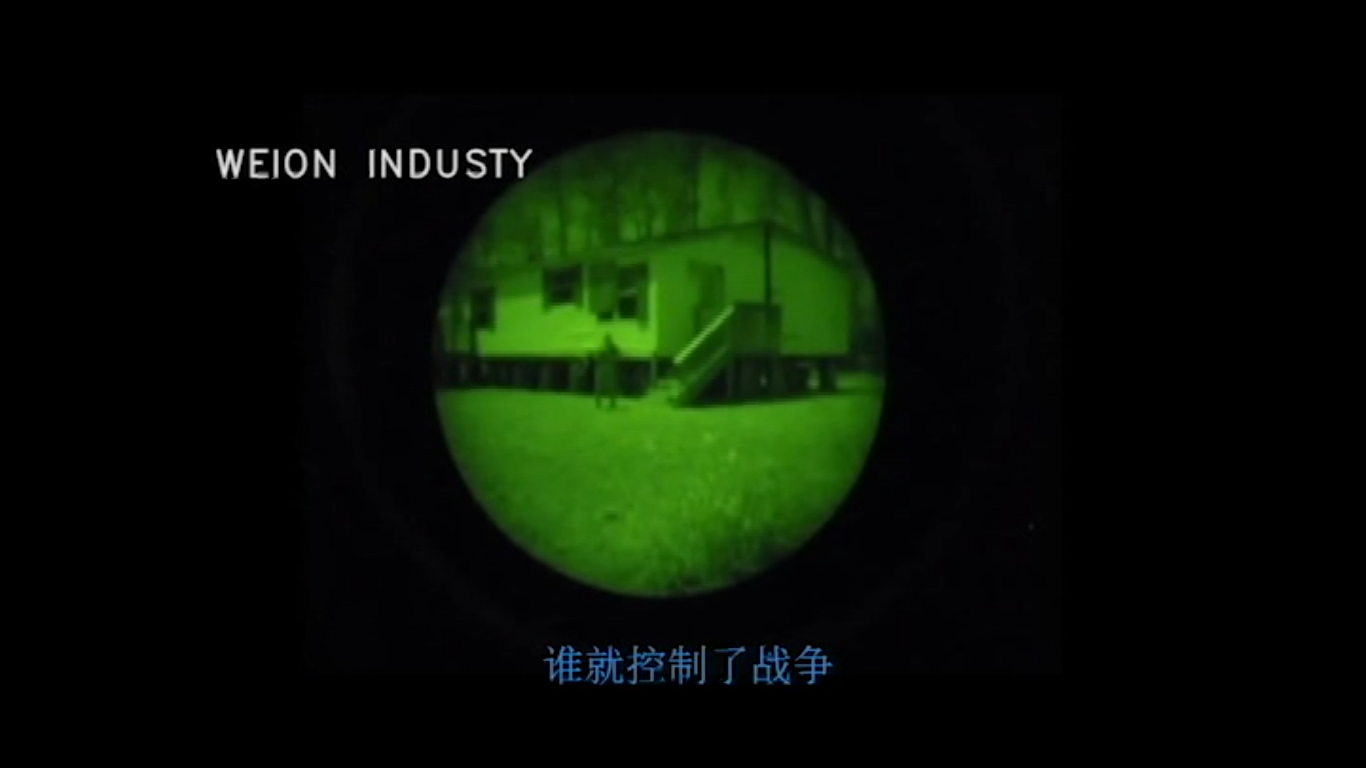
\includegraphics[
      width = \linewidth,
    ]{screenshot/30}
    \caption{0:30--0:31瞄准}%
    \label{fig:screenshot/30}
  \end{subfigure}

  \begin{subfigure}[htbp]{0.45\linewidth}
    \centering
    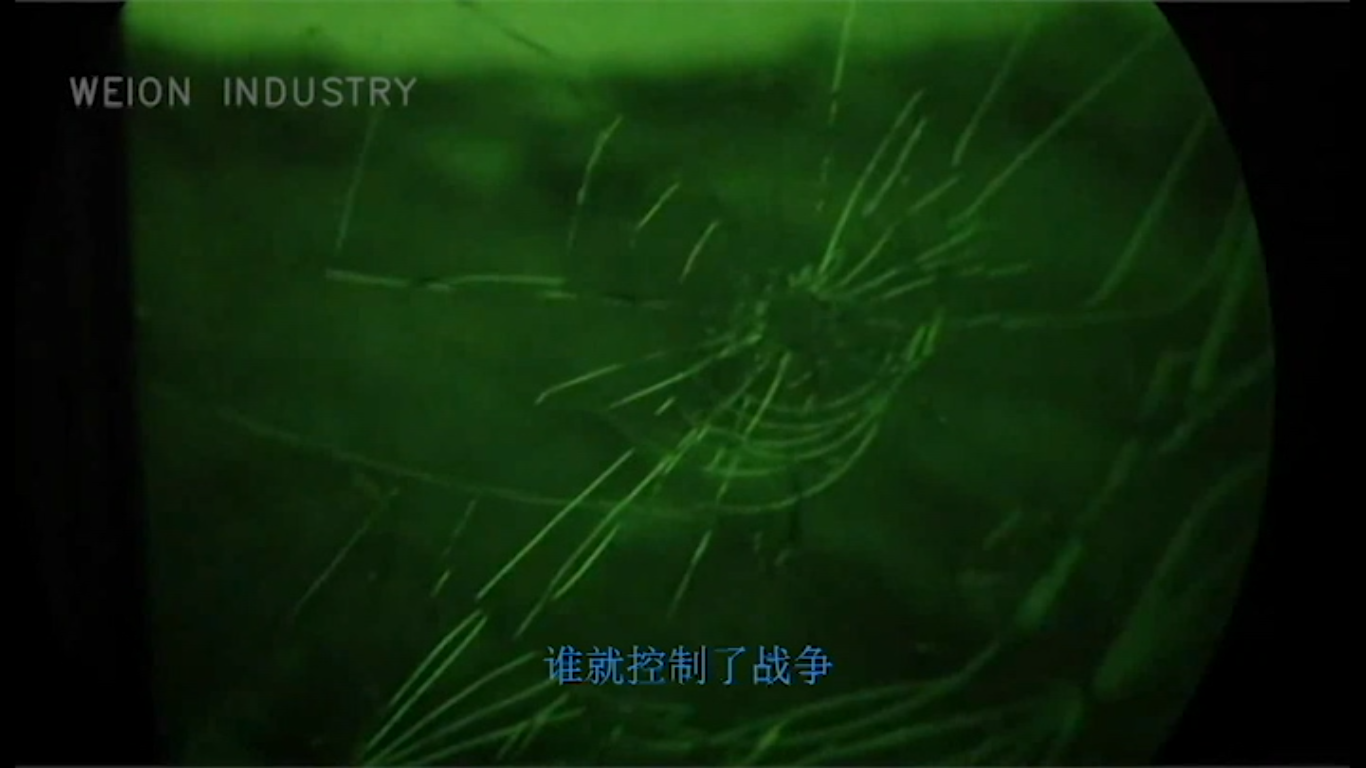
\includegraphics[
      width = \linewidth,
    ]{screenshot/31}
    \caption{0:31--0:32枪击}%
    \label{fig:screenshot/30}
  \end{subfigure}
  \caption{截屏}%
  \label{fig:screenshot}
\end{figure}

\section{夜视仪的3维爆炸动画}%
\label{sec:3d}

本视频中难度系数最高的地方。从网上下载一个夜视仪的stl 文件。用
\href{https://www.keyshot.com/}{Keyshot}得到其爆炸图。stl 是一种3D 打印机能
打印出的标准文件格式,可以从大多数3D 绘图软件中得到。
\href{https://www.keyshot.com/}{Keyshot}则是一种3D 渲染软件,可以模拟3维物体
在某种材质下的光照,得到渲染图或渲染动画,从而用做产品展示。

\section{夜视仪示意图}%
\label{sec:dia}

从答辩的PPT中截图得到图~\ref{fig:dia}。

\begin{figure}[htbp]
  \centering
  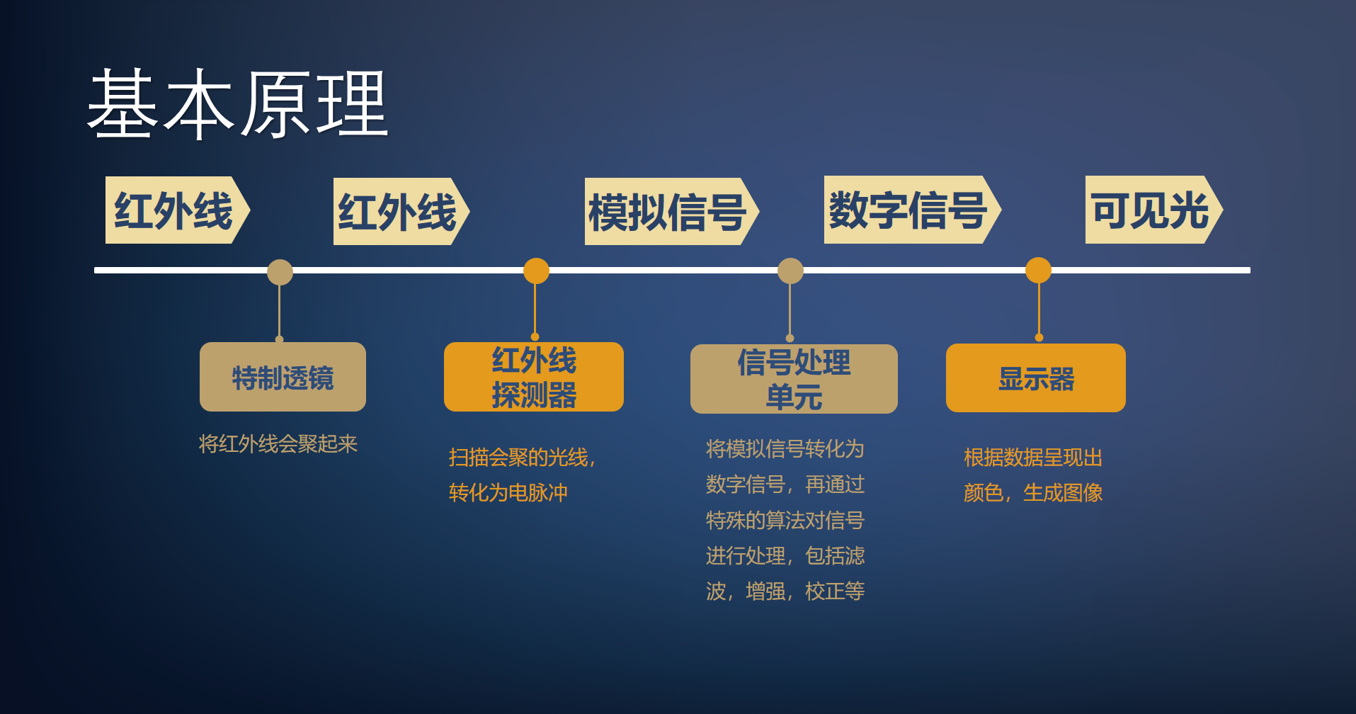
\includegraphics[
    width = 0.8\linewidth,
  ]{dia}
  \caption{基本原理}%
  \label{fig:dia}
\end{figure}

\section{校正算法对比图}%
\label{sec:compare}

从论文中截图得到图~\ref{fig:calibrate}。

\begin{figure}[htbp]
  \centering
  \begin{subfigure}[htbp]{\linewidth}
    \centering
    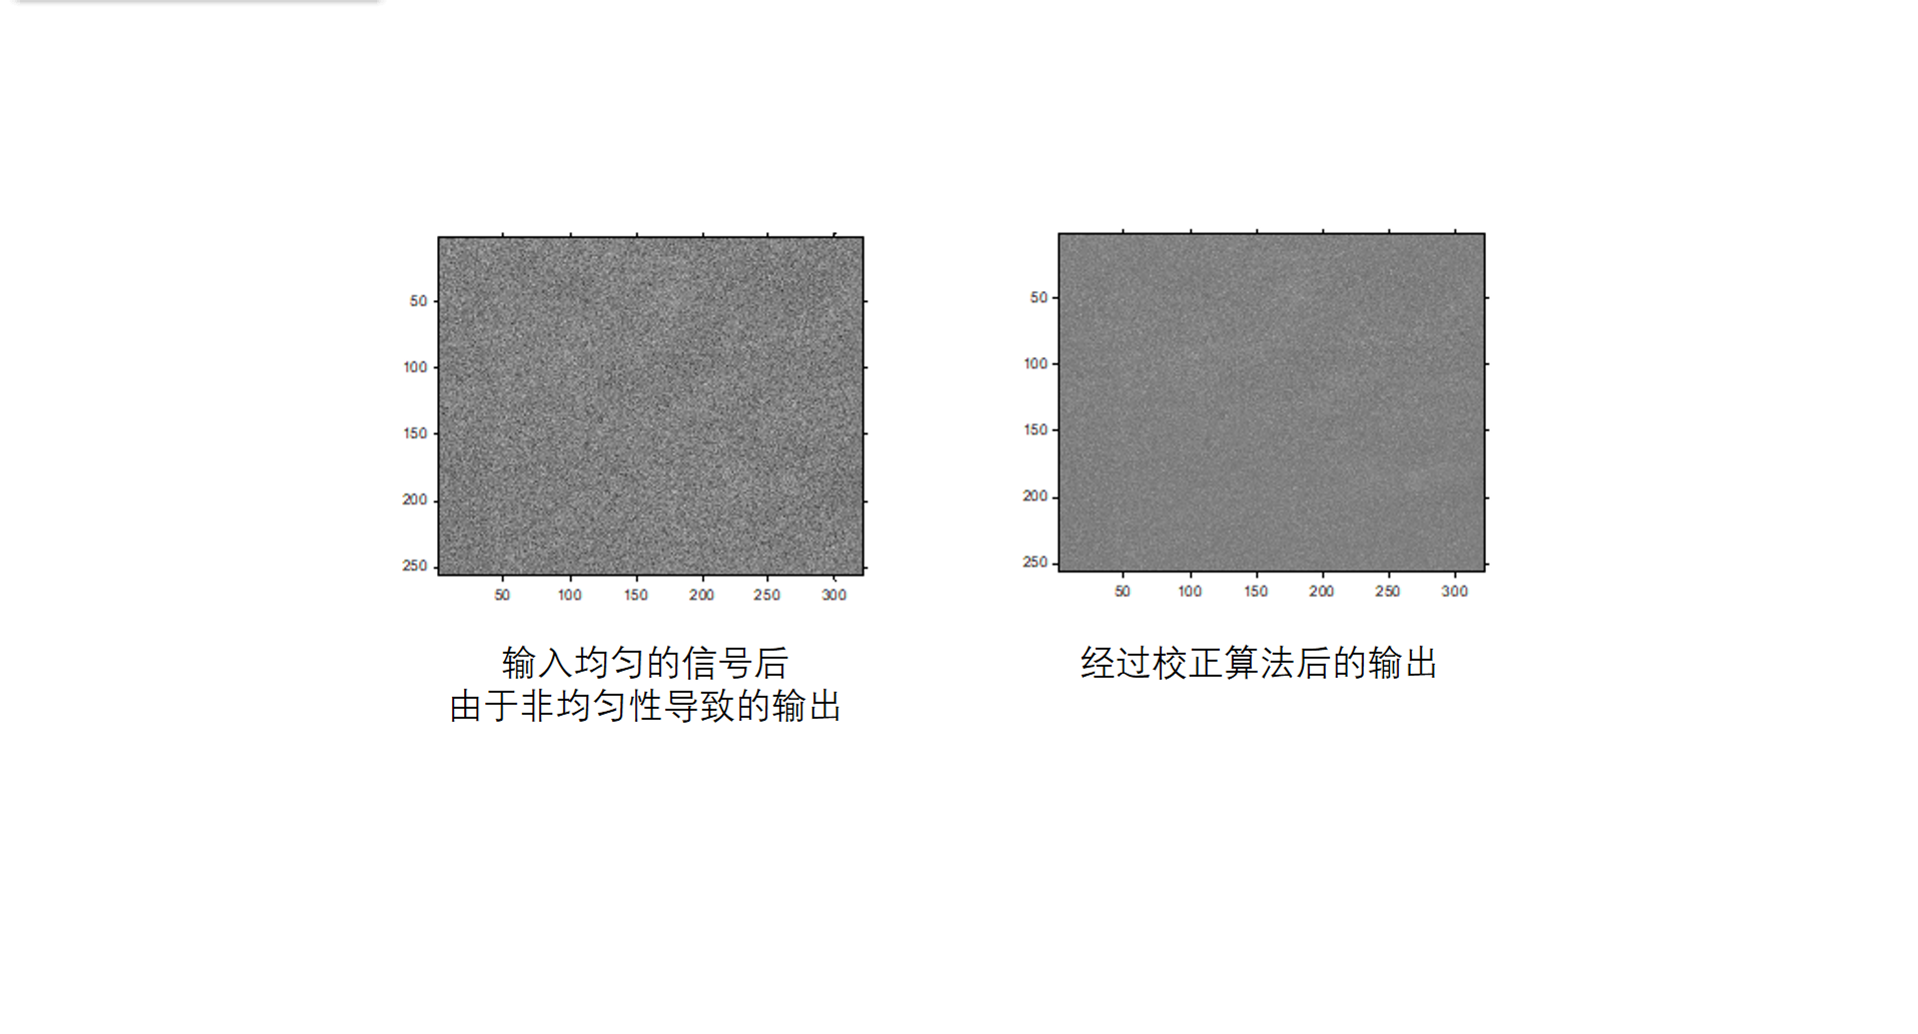
\includegraphics[
      width = \linewidth,
    ]{calibrate/1}
    \caption{校正算法对比图1}%
    \label{fig:calibrate/1}
  \end{subfigure}

  \begin{subfigure}[htbp]{\linewidth}
    \centering
    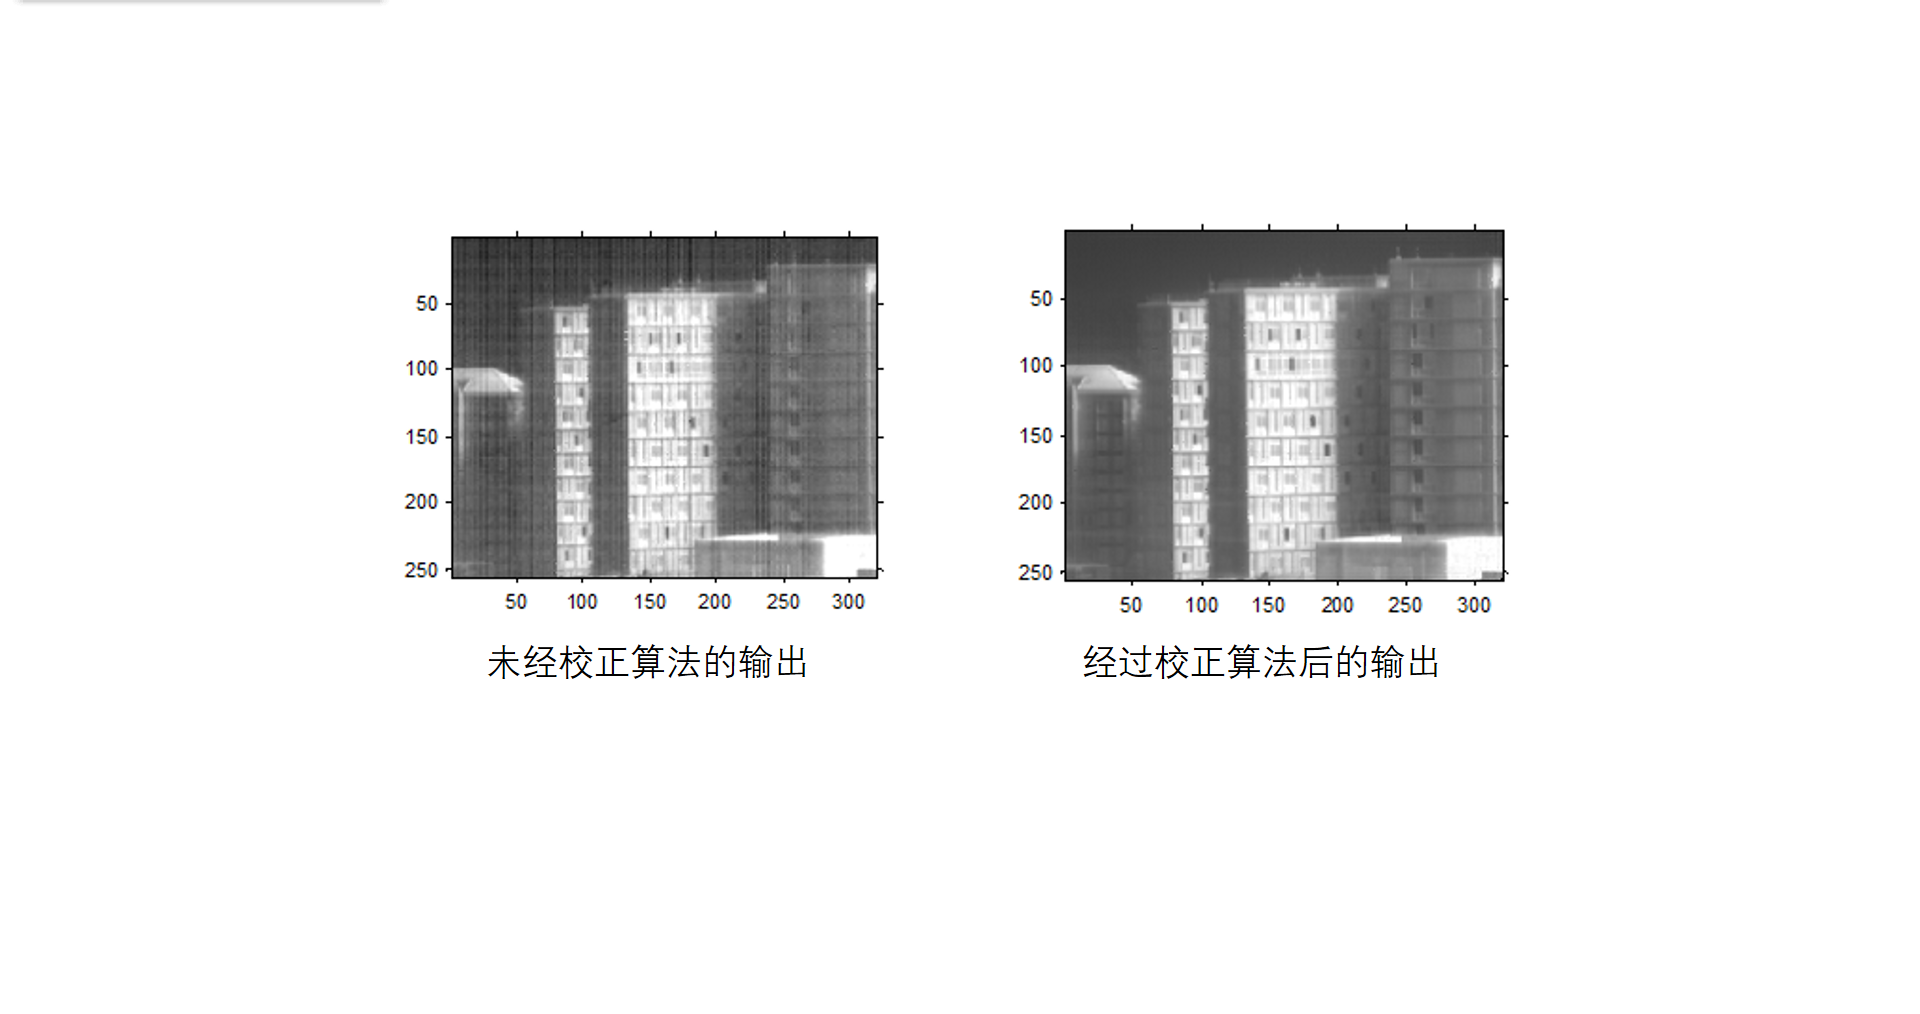
\includegraphics[
      width = \linewidth,
    ]{calibrate/2}
    \caption{校正算法对比图2}%
    \label{fig:calibrate/2}
  \end{subfigure}

  \begin{subfigure}[htbp]{\linewidth}
    \centering
    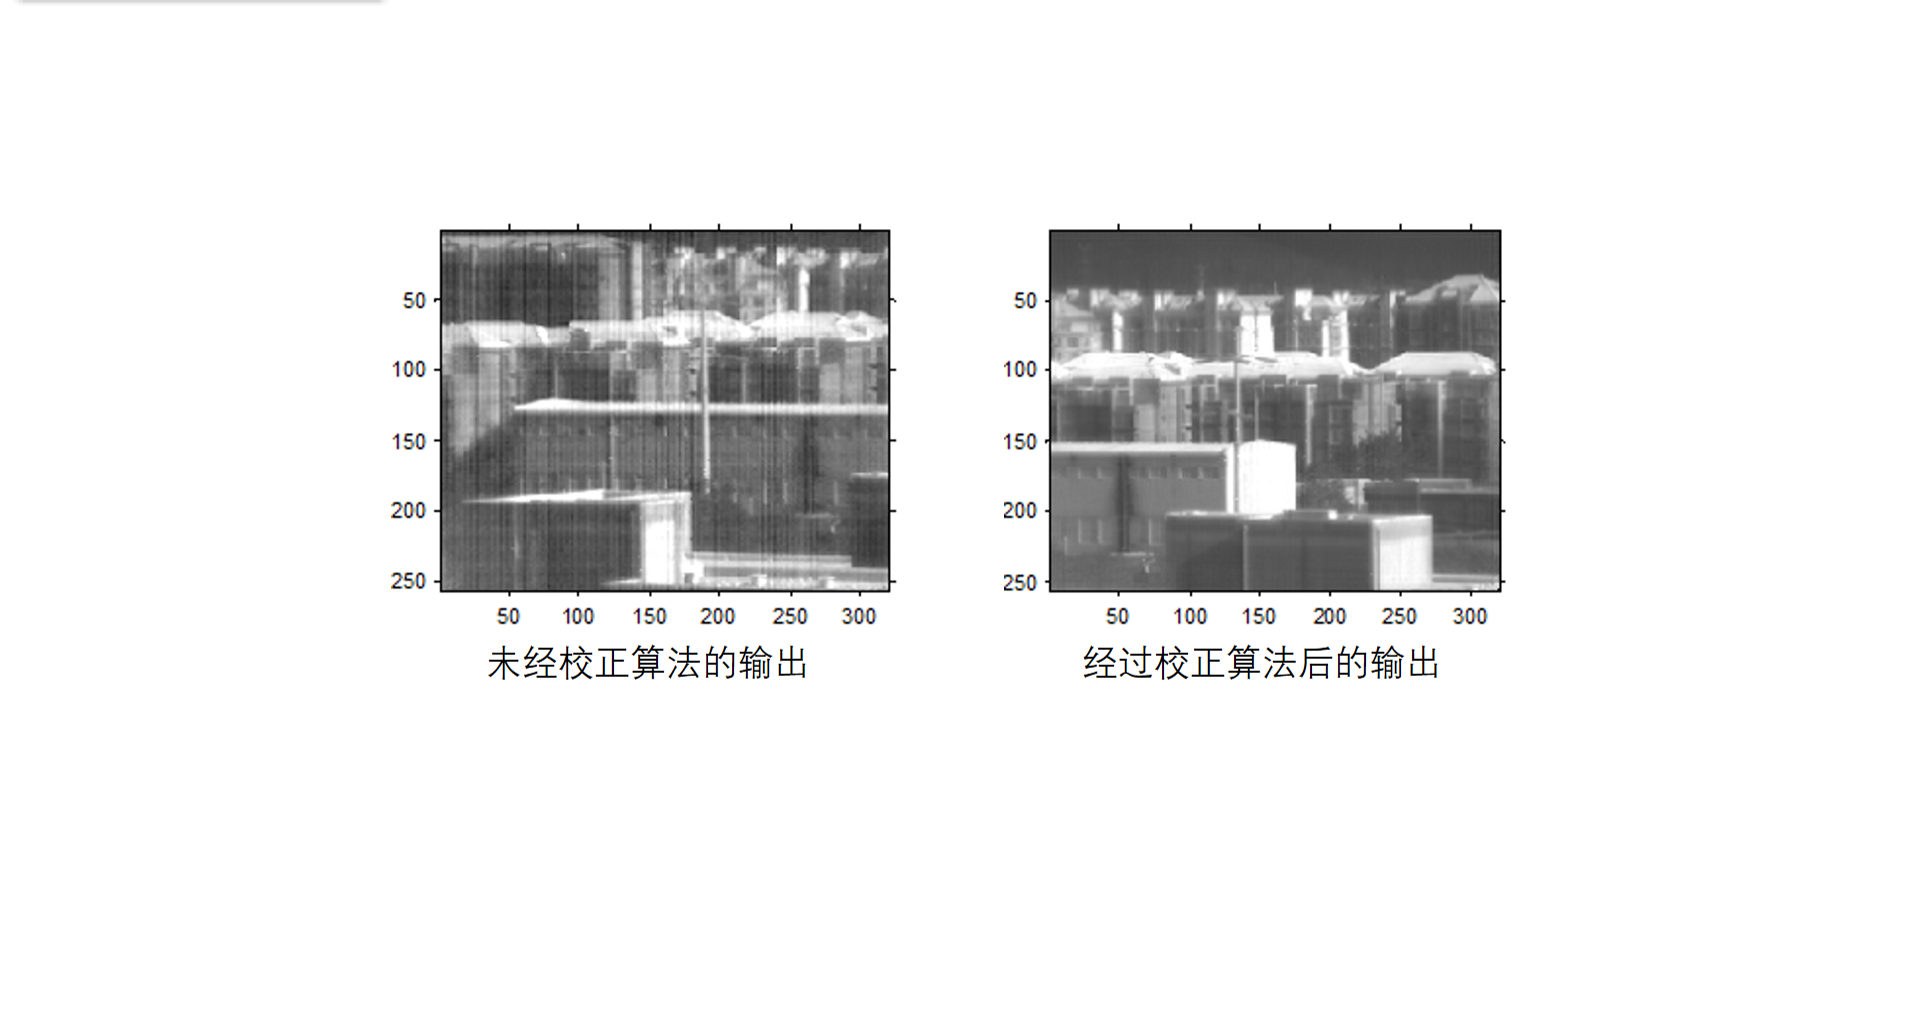
\includegraphics[
      width = \linewidth,
    ]{calibrate/3}
    \caption{校正算法对比图3}%
    \label{fig:calibrate/3}
  \end{subfigure}
  \caption{校正算法对比图}%
  \label{fig:calibrate}
\end{figure}

\section{甘特图}%
\label{sec:gantt}

利用\href{https://www.microsoft.com/en-us/microsoft-365/excel}{Excel}绘制图%
~\ref{fig:gantt}。

\begin{figure}[htbp]
  \centering
  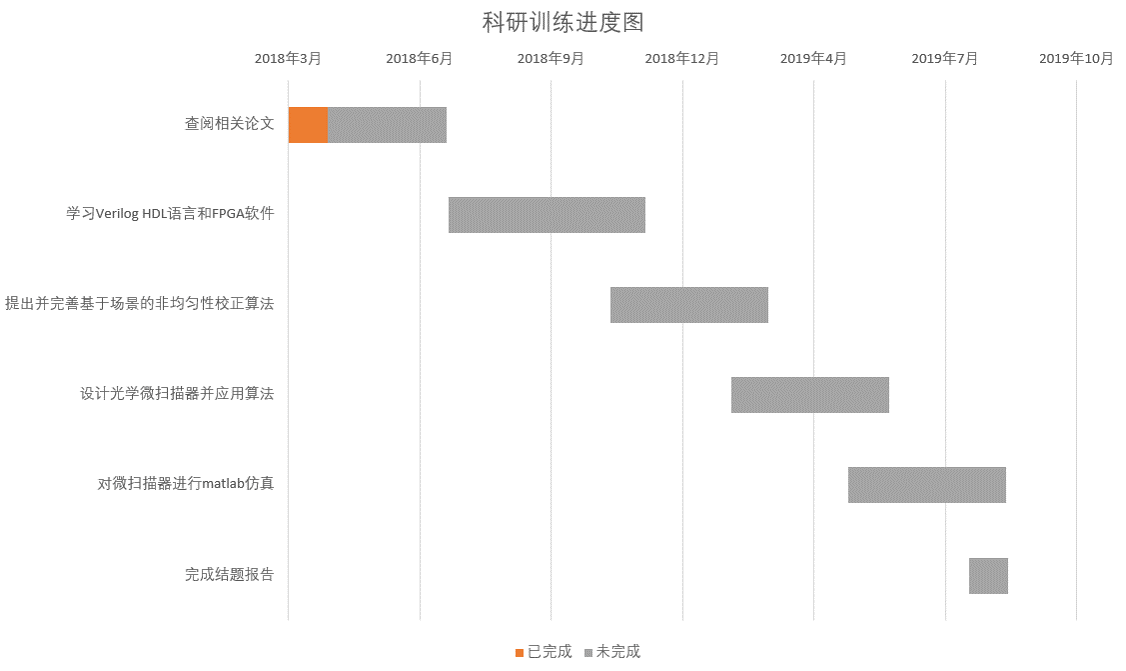
\includegraphics[
    width = 0.8\linewidth,
  ]{gantt}
  \caption{甘特图}%
  \label{fig:gantt}
\end{figure}

\end{document}

